% chercher des documents LaTeX dans styles, corps et bib
\makeatletter\def\input@path{{styles/}{corps/}{bib/}}\makeatother

%-------------------------------------------------------------------------------
%-------------------------------------------------------------------------------
% compiler avec pdflatex.
%for Latex project see: https://www.overleaf.com/learn/latex/Multi-file_LaTeX_projects.
%-------------------------------------------------------------------------------
%-------------------------------------------------------------------------------

% Utiliser le style rapport.cls
\documentclass[english]{rapport}


\setcounter{secnumdepth}{5} %paramètre la profondeur d'affichage des numéros de 
                            %sections...

% lettrine style
%\renewcommand{\LettrineFontHook}{\Rothdnfamily}
\renewcommand{\LettrineFontHook}{\calligra}

\title{2019 Summer Internship\\
Dalhousie University, Halifax, Nova Scotia, Canada\\
\rule{\textwidth}{1pt}
\\\textit{Robust Deep Learning Tracking Robot\\}
\rule{\textwidth}{1pt}
}
\author{
written by \textsc{Arnaud Klipfel}, Robotics specialization at \textsc{ENSTA-Bretagne}\\
supervised by Dr. \textsc{Thomas Trappenberg, Dalhousie University}
 }
\date{\today}
\doctype{report}
\promo{CI2020\\second year}
\etablissement{\textsc{Ensta} Bretagne\\2, rue François Verny\\
  29806 \textsc{Brest} cedex\\\textsc{France}\\Tel +33 (0)2 98 34 88 00\\ \url{www.ensta-bretagne.fr}}
\logoEcole{
\includegraphics[height=4.2cm]{logo_ENSTA_Bretagne_Vertical_CMJN}} % enables the import of the logoecole variable in the forepage.
\logoOtherEcole{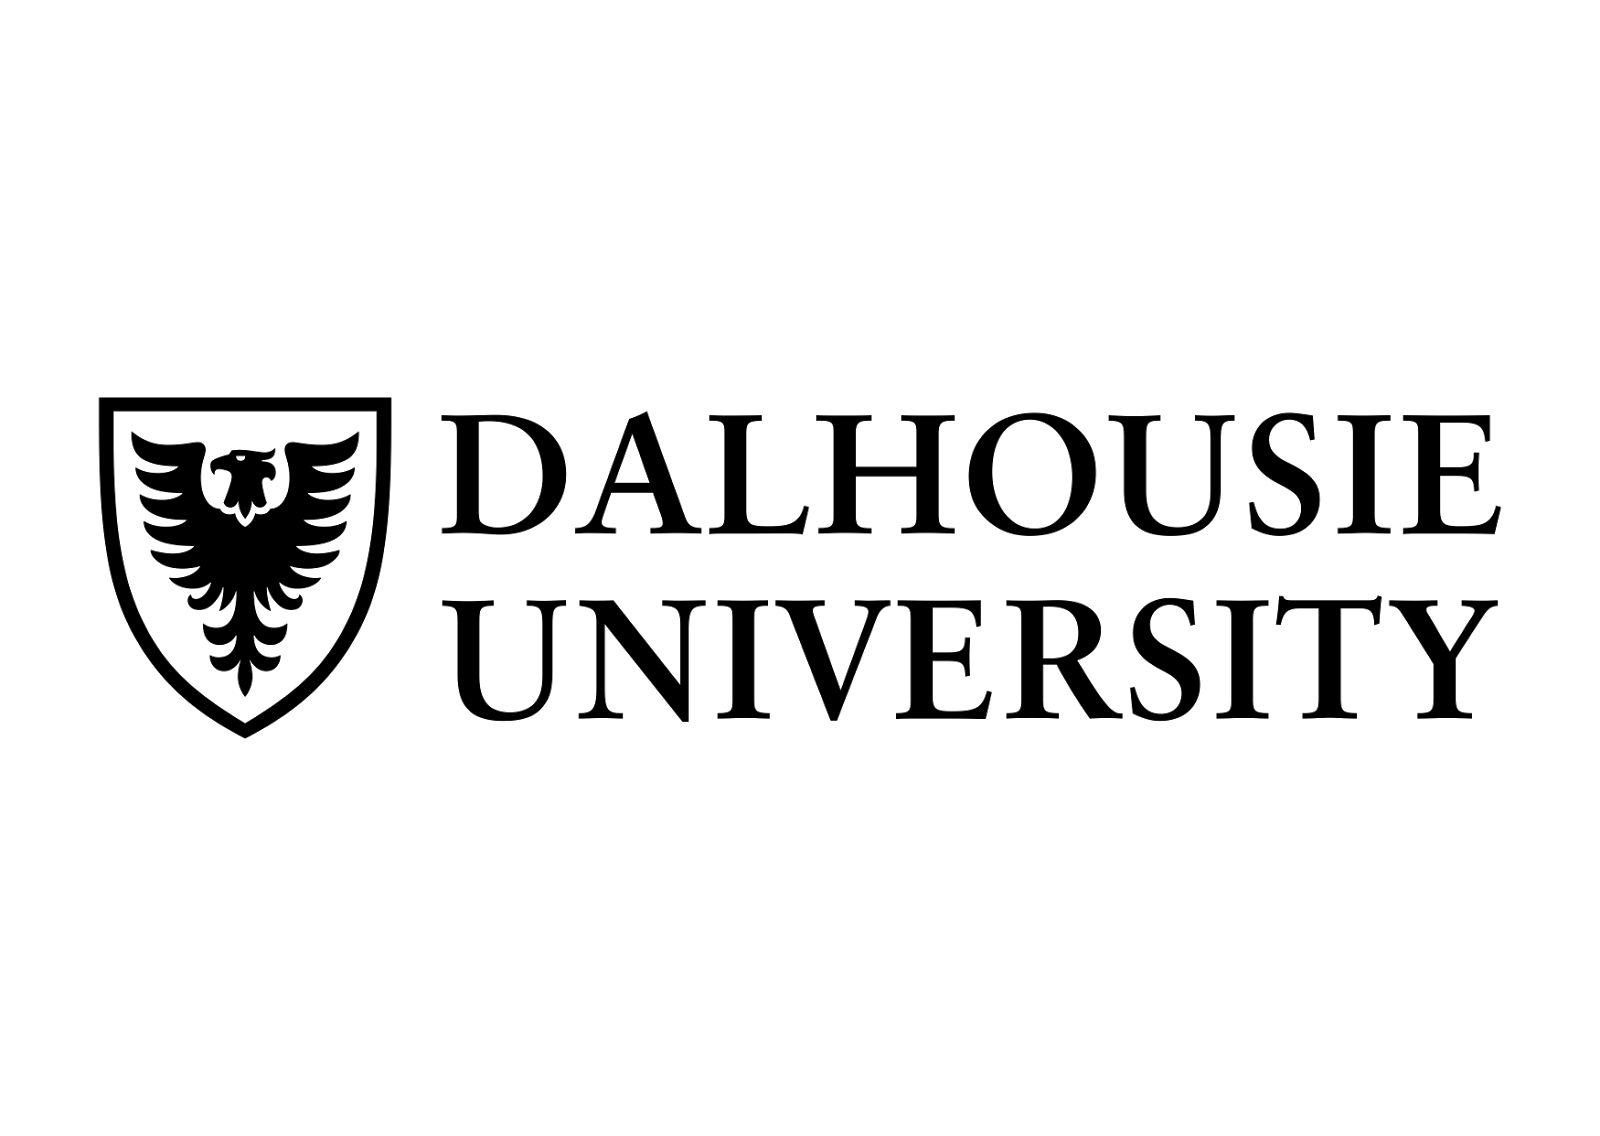
\includegraphics[height=3.6cm, width=4.0cm]{logo_dal_nd.png}}
% creer l'index
\makeindex

\begin{document}
\selectlanguage{english}
% creer le titre ici
\maketitle
\tableofcontents
\clearpage
% chargement du fichier abstract.tex
% chargement du fichier corps.tex`

\vspace{50pt}

\section*{Ackowledgement}\label{thk}

This internship was a very enriching experience in my life.
Undoubtedly, the concepts and tools I have come to learn will 
guide me in my future research career. I want to deeply thank
Dr. Trappenberg for his astute and lasting support
in my work.


\clearpage

\section*{Abstract}

% VERIF : *
\introductionLettrine{T}{he} concept of tracking robot can bring trailblazing and 
game-changing applications either in the industry, defense or
at home. More practically, robots could be seen as
the future coworkers of humans. In that context, 
robots will have at some point to be able to 
not only follow instructions, but assist for instance
workers in a factory, and so be able to 
follow their track. One can imagine a robot that could 
carry tools, follow any worker, and hand out the right one 
when asked.
\\\indent Few trackers following general targets, not just 
human ones, have been realized using deep learning
techniques, and even fewer using the middleware
\textit{ROS}. As a matter of fact, this project aimed to 
realize a versatile \textit{ROS} architecture
for a tracking robot using a stereo camera
and deep learning algorithms to spot a 
general given target.
\\\indent The project was divided into 
several main stakes. First of all, the hardware
of the tracker had to be wisely selected to 
meet the requirements of the tracking process. 
Secondly, the tracking algorithm had to be chosen 
and assessed. The \textit{ROS} architecture had 
then to be imagined and built. Finally, the thorniest 
part was to integrate each part on the robot.
\\\indent At the end, a flexible and general \textit{ROS}
architecture was implemented and tested in diverse 
conditions. The realized architecture 
could then inspire future work, and be the basis 
of some improvements thanks to the flexibility of \textit{ROS}.


\clearpage
\section*{Introduction}
% VERIF : *
\introductionLettrine{T}{his} document is the report of the project on which 
I worked during my summer internship in 2019 at Dalhousie 
University. Additional codes and documentations
could be found on my personal \href{https://github.com/klipfel}{\textit{github}}.
The main goal was to build a tracking robot
with the middleware ROS and with deep learning techniques.
\\\indent The part \vref{context} contextualize the project, 
presents the goals and the strategy. The part \vref{stateofart}
outlines several projects or existing techniques that 
were relevant for the project in any way. The part 
\vref{hardware} explains how the hardware of the 
tracker was selected. The part \vref{software}
justifies the choices made regarding the 
tracking algorithm and the \textit{ROS} architecture.
The part \vref{results} analyzes the results of the integration
of each single part on the robot, that is to say the hardware and 
the software. Finally, the part \vref{setup} gives the procedure 
and some pieces of advice in order to replicate the latest blueprint
of the tracker.

%\section*{Abstract}
\section*{Keywords} stereo-vision, tracking, \textit{ROS},
mechatronics, mobile robotics, RC car, ground robot, deep learning.

%\selectlanguage{french}
%\section*{Mots clés}


%%% Local Variables: 
%%% mode: latex
%%% TeX-master: "../guide"
%%% End: 

\clearpage
\newgeometry{hmargin=2.5cm,vmargin=2cm}

\chapter{Project Contextualization}

	\section{Project Specification}
	
		\subsection{Motivations}
	
		The main goal of this project was to build a \textit{Deep Learning Tracking Robot}. Many tracking
		robots have been implemented in the previous years, few have used the adaptive, versatile, and 
		now standard robotic Middleware \textit{ROS}\footnote{Which stands for \textit{Robot Operating System}.}.
		\\\indent Why \textit{ROS} precisely? As defined by Anis Kouba in \cite{latexcompanion}, \textit{ROS}
		is an \frstg{} open-source \textit{middleware} \lstg{} that provides a robust and reliable framework 
		to build robots. \textit{ROS} is a voguish tool to create robots with advanced functionalities so much so 
		that it has become the standard to develop robots. \textit{ROS2} is already in part 
		operational. In this project though, 
		it has been decided that the first version of \textit{ROS} will be used since \textit{ROS2} is still 
		in heavy development and \textit{ROS} is better documented than its counterpart.
		\\\indent Why is \textit{Deep Learning} suitable for robotic applications? In general, \textit{AI}
		\footnote{Artificial Intelligence, which comprises \textit{Deep Learning}.}
		is really adapted for critical algorithms, such as embedded codes
		on robots, since the performances are much higher than with traditional implementations. By traditional
		implementations, one could for instance consider iterative algorithms where for a particular task 
		all processes are hand-implemented. \textit{AI} enables much finer and more robust
		implementations since the \textit{model},
		which can be regarded as the applied processes, can evolve by itself through diverse methods such as training.
		 
		\subsection{Requirements}
		
		In order to realize the tracking robot, several requirements had to be met in this
		project. First of all, the robot had to reuse an old \textit{Race Car} platform comprising
		the chassis, the wheels \dots all the mechanics. The brain of the robot, that is to say
		the embedded computer will be the \textit{Jetson Nano} designed by \textit{Nvidia}. By and
		large, to build the tracker the material of the laboratory had to be used as much as 
		possible, and the equipment bought had to remain affordable.
		%TODO image of the old platform rc car
		%TODO image of the jetson nano
	
	\section{Strategy}
	
		\subsection{Different periods}

		Developing a robot is a critical task, and has to be conducted thoroughly. 
		In this regard, \textit{ROS} builds a framework for developing 
		robots in a more organized way. For each task to implement, 
		the work-flow has always been the following: research, simulation, isolated 
		tests, integration.
		\\\indent Before even implementing something and integrating it, one should 
		research all the possibilities that are offered to them. Then one of the 
		easier or maybe most sustainable options could be chosen. Yet, even the
		tests, simulation, and integration has to be thought and foreseen beforehand.
		\\\indent Simulating robots, without depending on the hardware is
		a needed step.	 A specific hardware has always some specificities that
		could hide some issues and unpredictable behaviors. As a matter of fact, 
		simulating algorithms that will be integrated in the robot afterward in 
		a controlled environment prevents any hardware based issue to shadow
		our understanding of the basic implementation of
		the \textit{software}.
		\\\indent Once the simulation is in place, it is then 
		recommended to test the simulation as much as possible in order
		to unveil some detrimental singularities. In the case of the hardware, 
		each component has to be tested independently before integration
		\footnote{Especially, some driver issues are sometimes really 
		hard to pinpoint.}.
		\\\indent The final step is to integrate the work in the robot, and
		to test it to see if the robot behaves as expected or if there 
		is any regression.
		\\\indent A robot is not just a piece of software, it is a system 
		where the interaction of the software and the hardware is by 
		definition the future behavior of the robot.
		
		\subsection{Different aspects}

		The development of a robot encapsulates different areas or type of work.
		In the construction of the tracker, principally two aspects 
		have been tackled, the hardware, and the software.
		\\\indent In the first place, the hardware has to be well-chosen beforehand.
		The motor had to replaced, the \textit{wifi} access had to be added, batteries 
		had to be chosen \dots to fit the requirements of the tracking robot.
		\\\indent In the second place, the sofware has to be implemented. Precisely, 
		the tracking algorithm had to be chosen, and the \textit{ROS} architecture had 
		to be designed.
		
\chapter{State of the art}

		In order to build the tracker, the first step was to choose the
		hardware of the robot. Secondly, the \textit{ROS} architecture had to be decided
		and thirdly the tracking algorithm had to be implemented. This part 
		presents a brief overview of different existing projects and solutions 
		that could have been selected throughout the project. All the projects
		presented and listed here will then be compared and the choices
		made will be underpinned in the parts \vref{hardware} and \vref{software}.
		
		\section{Building an electric car}
		
		Several projects have aimed to realize an electric car robot, sometimes autonomous. 
		Having in mind these projects can give some piece of advice on how it is common 
		to design such systems.
		\\\indent Some projects have used the on-board computer \textit{Jetson Nano}. 
		One can name the following robots : \textit{Jetbot} \cite{jetbot}, \textit{Kaya} \cite{kaya}.
		These robots are both designed by \textit{Nvidia}, the designers of the 
		\textit{Jetson} board series\footnote{Jetson Nano, Xavier, TX1, TX2 \dots}. It 
		is notably interesting to take as example their hardware selection since they
		use the same embedded computer the tracker use.
		
		\section{Using ROS}
		
		
		
		\section{Tracking}
		
		
\chapter{Hardware}\label{hardware}

\chapter{Software}\label{software}
\clearpage

\section*{Conclusion}

\begin{comment}
	
	Compare to the paper on the person following which had a 20 Fps. (check whether or not they did it in c++)
	What has been implemented and what has not been implemented.
 E	Ideas for further development : ROS2, c++

\end{comment}

\introductionLettrine{T}{he} tracker robot was able to track 
a specified target, human targets were followed 
more accurately. The \textit{ROS} architecture
that has been implemented is flexible and could
be used for further improvements.
\\\indent Regarding the performances, in 
comparison to a person following robot \cite{personfollowing}
tracking at a rate of 20 \textit{FPS}, the tracker
implemented in this project tracks at a maximum of 6 \textit{FPS}.
The performances could be improved though. The person 
following robot was implemented in \textit{C++} in 
comparison to the tracker in this project, which was 
implemented entirely in \textit{Python}.
\\\indent It is also important to mention that not 
all the components ordered, and presented on 
figure \vref{hardwarepng}, had arrived before
the end of the project. Having the best components would 
have certainly improved the performances
of the tracking robot. Especially, the tracker 
would need to be tested with the \textit{Krisdonia 25000mAh}
power bank and the \textit{Intel 8265 Wifi module}.
\\\indent Another point of refinement could be the 
training of the \textit{GOTURN} model to make 
it more accurate, the realization of a personal 
deep learning network, or the test of another one.
\\\indent For any further implementation, 
and especially if realizing a personal 
deep learning model is the goal, switching to \textit{ROS2}
could be a wise move, since \textit{ROS2}
is coded in \textit{Python 3}, and would make it easier to 
use the common deep learning libraries out of the box, such 
as \textit{PyTorch} or \textit{Tensorflow}. 
For any deep learning implementation with the \textit{Jetson Nano}, 
it is recommended to read through the \textit{Nvidia} tutorials  first\cite{dptuto}.
\\\indent To sum up, the latest tested prototype, as presented in the \href{https://github.com/klipfel/tracker-v1}{github},
did not implement the speed control. The idea was to obtain first acceptable performances
for the tracking algorithm, which is the juggernaut of the robot. Several 
things should be tested for any motivation to continue this project:
\begin{itemize}
	\item[\textbullet] Transpose the \textit{ROS} architecture in \textit{ROS2}: it would then 
	be easier for any \textit{Python} support.
	\item[\textbullet] Implementing in \textit{C++}: the performances of
	\textit{C++} compared to those of \textit{Python} are unequivocal. The \textit{Jetson Nano}
	was designed to be more suitable for \textit{C++} programming. It would be more
	flexible for \textit{GPU} acceleration.
	\item[\textbullet] Hard-code the tracking model in \textit{PyTorch, tensorflow}, so that 
	it would be possible to use \textit{GPU acceleration} on the \textit{Jetson Nano}, cf. 
	integration presented in \vref{test4}. The code of the \href{https://github.com/klipfel/tracker-v2}{prototype 2}
	could be used as a start.
	\item[\textbullet] Test the \textit{Wifi} module and the \textit{Krisdonia 25000mAh}
	of the \textit{ROS} architecture 
	presented in \vref{hardwarepng}, when delivered.
	\item[\textbullet] Test the speed control as presented in figure \vref{rosarchitecture} and in \vref{speed}.
\end{itemize}

\appendix

\chapter{Hardware Library}\label{hardwarelib}

\lstset{language=Python}
\lstinputlisting[language=Python, caption = {Hardware library : file \textit{hardware.py}}]{codes/hardware.py}

\chapter{ROS}

\clearpage
\phantomsection
\addcontentsline{toc}{chapter}{Bibliography}
\printbibliography
\end{document}

%%% Local Variables: 
%%% mode: latex
%%% TeX-master: t
%%% End: 
